\subsection{Beyond Basic FNNs}

The general application area for NNs is supervised learning. This has been the focus and most dominant usage.
\begin{itemize}
  \item This creates the requirement of labeled data as input, potentially a large amount of those
  \item There is a huge variety of network types, as we saw before, also optimized for different input types:
  \begin{itemize}
    \item CNNs use convolution to better deal with images
    \item RNNs and LSTM (Recurrent NN, Long Short-Term Memory) are tailored for temporal or sequential data
  \end{itemize}
  \item Generally, NNs require lots of engineering and trial and error \begin{note}(no magic bullet, no free lunch)\end{note}
\end{itemize}

Beyond supervised learning, there are also \textbf{unsupervised learning} applications, where we don't use classes or similar things as our target.

For example, in the case of \textbf{autoencoders}\sidenote{Autoencoder}, the "label" is produced from the input such that the input is tried to be reproduced. The error is the difference between input and calculated output. The interesting part is the significantly more dense representation of the input data captured by the middle layer, as can be seen in \ref{fig:6_bb_autoencoder}.

\begin{figure}[H]
  \centering
  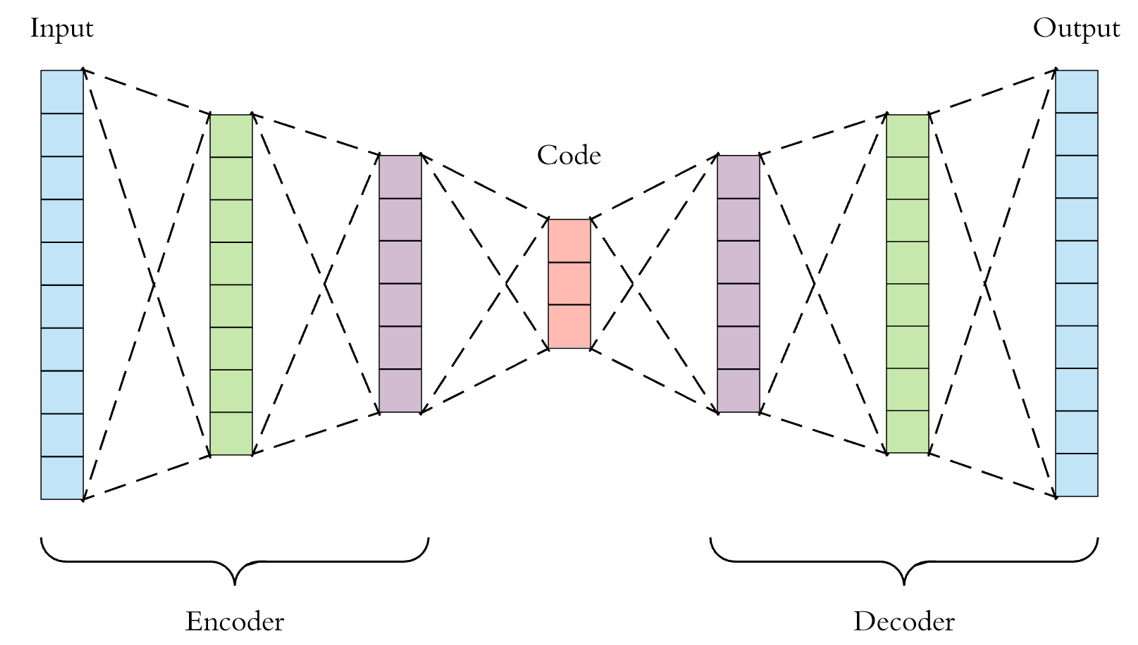
\includegraphics[width=0.6\textwidth]{assets/nn/in__auto_arch.png}

  \vspace*{0.5cm}
  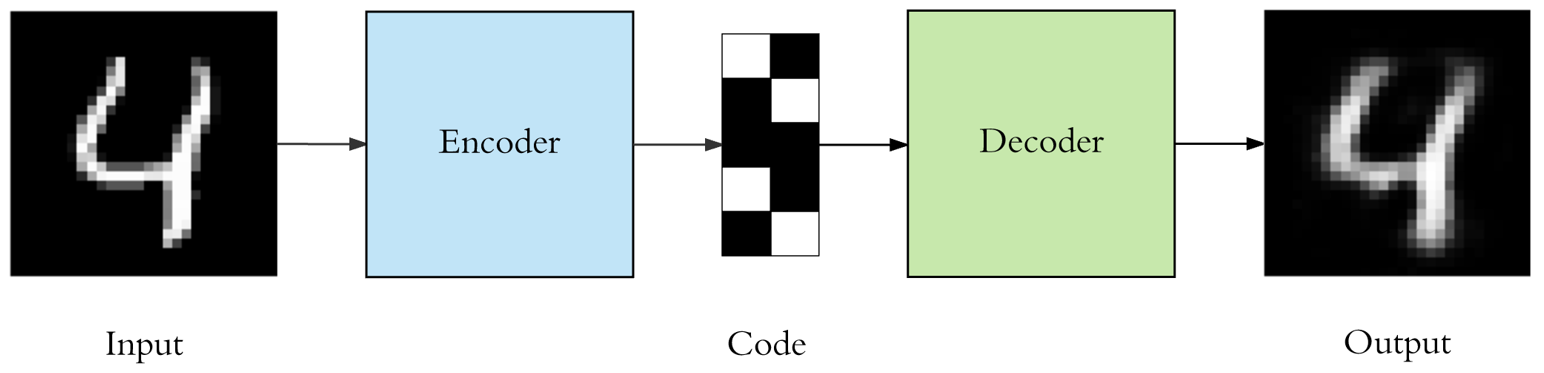
\includegraphics[width=0.7\textwidth]{assets/nn/in__auto_code.png}
  
  \caption{Unsupervised learning: autoencoder}
  \label{fig:6_bb_autoencoder}
\end{figure}

Another application is \textbf{GANs}\sidenote{Generative Adversarial Networks} (generative adversarial networks). Here, we have two networks:
\begin{itemize}
  \item One network is the generator that tries to create "fake data" (e.g. fake art, fake people)
  \item The other is the discriminator that tries to distinguish "real" from "fake data"
  \item This means, they have opposing goals
\end{itemize}

\begin{figure}[H]
  \centering
  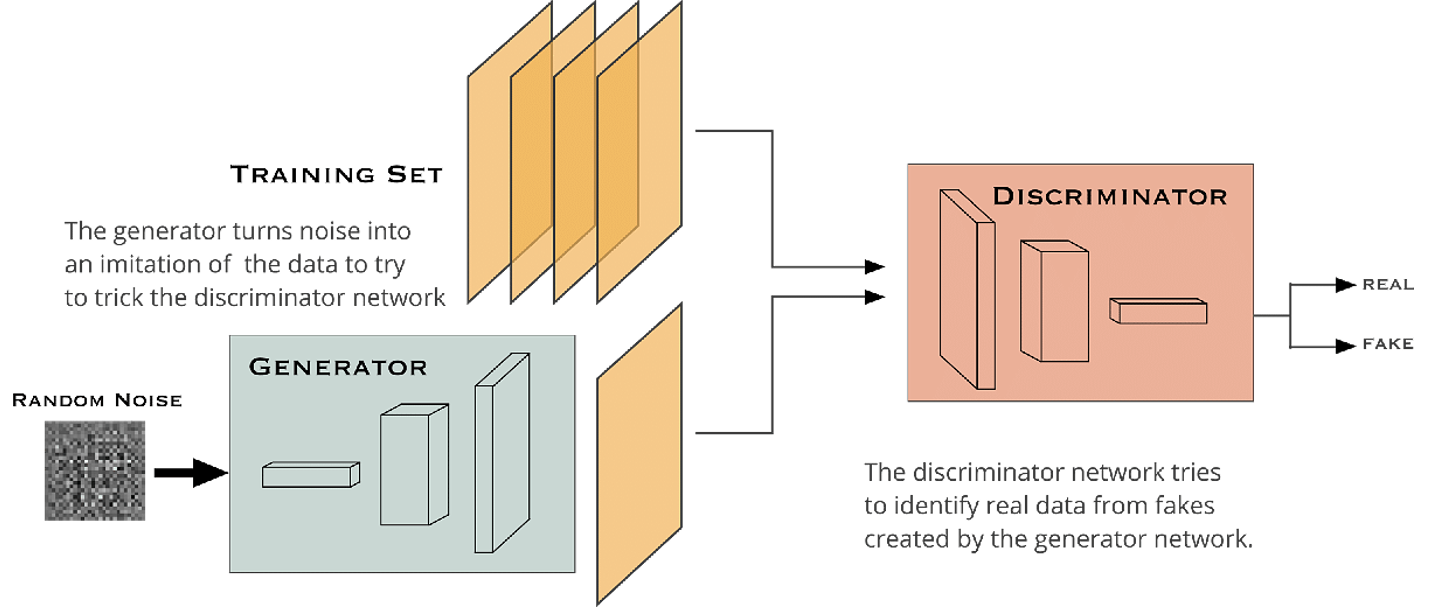
\includegraphics[width=0.7\textwidth]{assets/nn/bb__gan.png}

  \vspace*{0.5cm}
  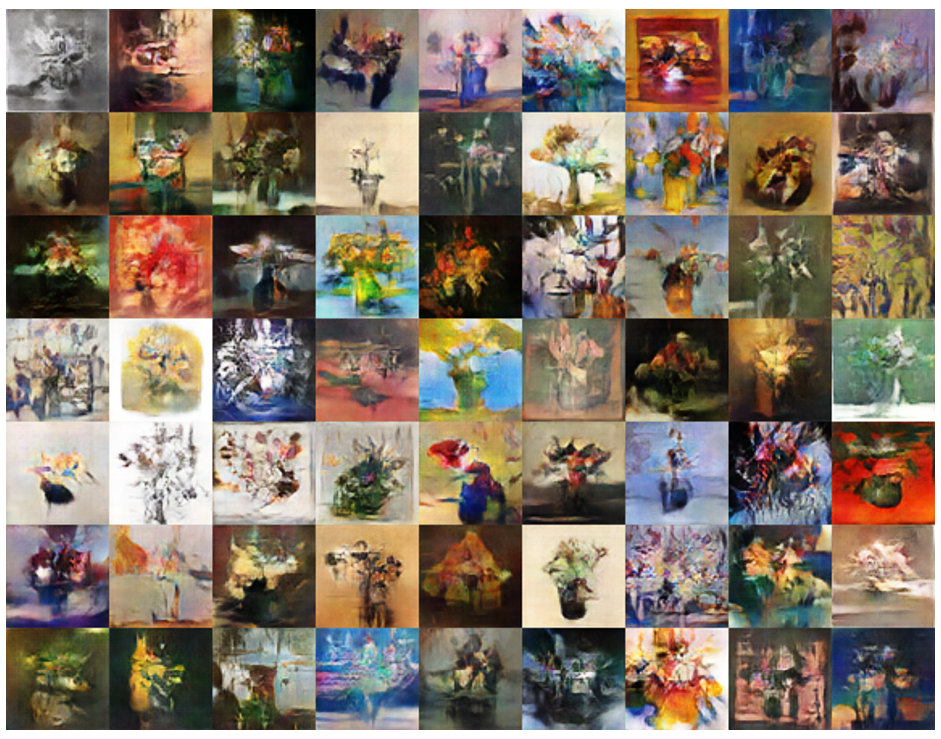
\includegraphics[height=3.5cm]{assets/nn/bb__gan_res.png}
  \hspace*{0.5cm}
  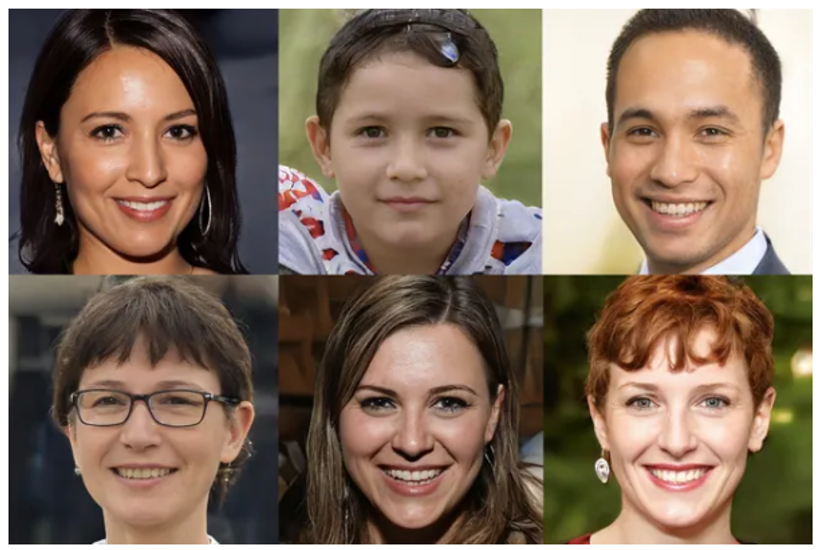
\includegraphics[height=3.5cm]{assets/nn/bb__gan_res_2.png}
  
  \caption{Unsupervised learning: GANs}
  \label{fig:6_bb_gan}
\end{figure}

A final unsupervised application is \textbf{self-organizing maps}\sidenote{Self-organizing maps} which is a directly unsupervised neural network.
\begin{itemize}
  \item We have a distribution of the training data \begin{note}(blue blob)\end{note}
  \item In the beginning, the SOM nodes are arbitrarily positioned in the data space
  \item Then the following process is iterated until all input data has been seen:
  \begin{itemize}
    \item Randomly select a training data point as input \begin{note}(white point)\end{note}
    \item The node nearest to the training node is selected as winner \begin{note}(yellow point, with neighbors in yellow area)\end{note}
    \item It is then moved toward the training data, just as the neighbors on the grid (just to a lesser extent), so update the neurons
  \end{itemize}
  \item Then the input can be classified
  \begin{itemize}
    \item The inputs are connected to the neurons with weights
    \item The neurons are also related to each other
  \end{itemize}
\end{itemize}

\begin{figure}[H]
  \centering
  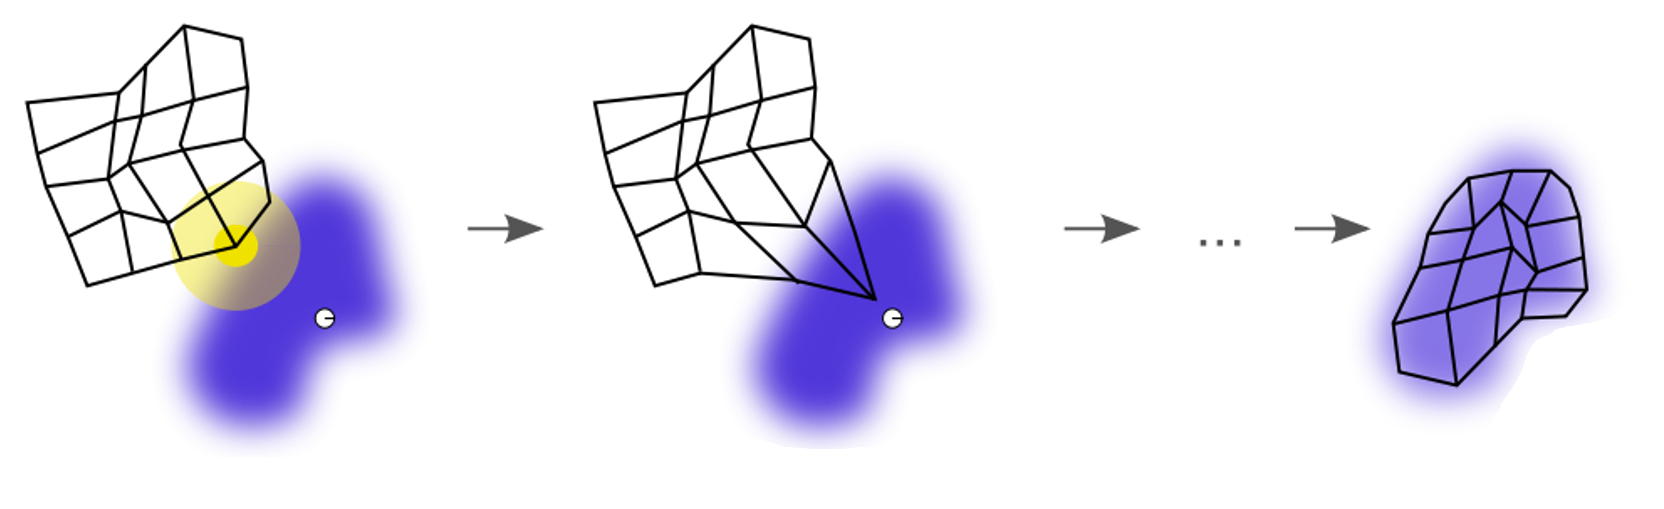
\includegraphics[width=0.6\textwidth]{assets/nn/bb__som.png}

  \vspace*{0.5cm}
  \begin{subfigure}{0.6\textwidth}
    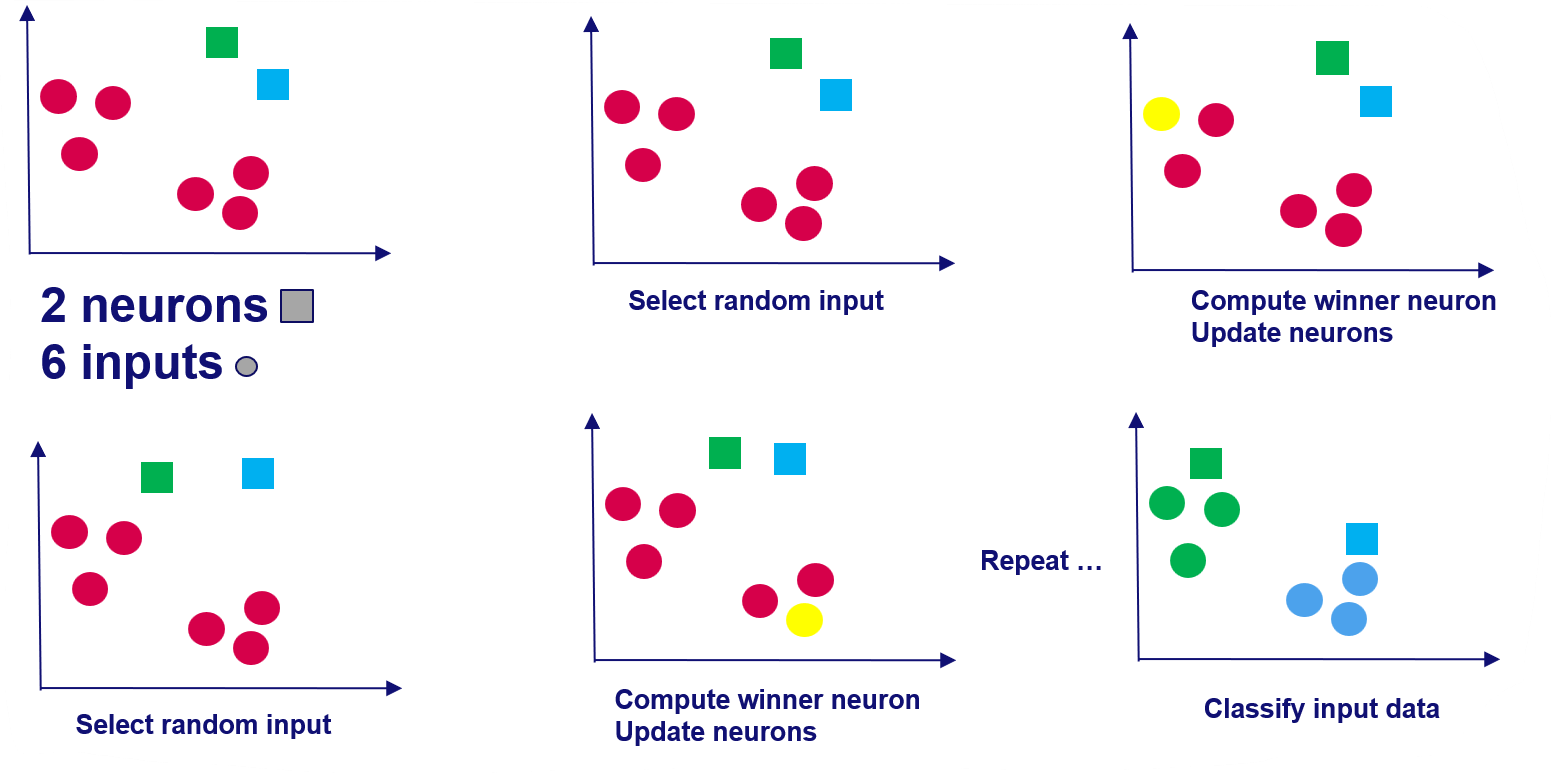
\includegraphics[width=\textwidth]{assets/nn/bb__som_ex1.png}
  \end{subfigure}

  \vspace*{0.5cm}
  \begin{subfigure}{0.6\textwidth}
    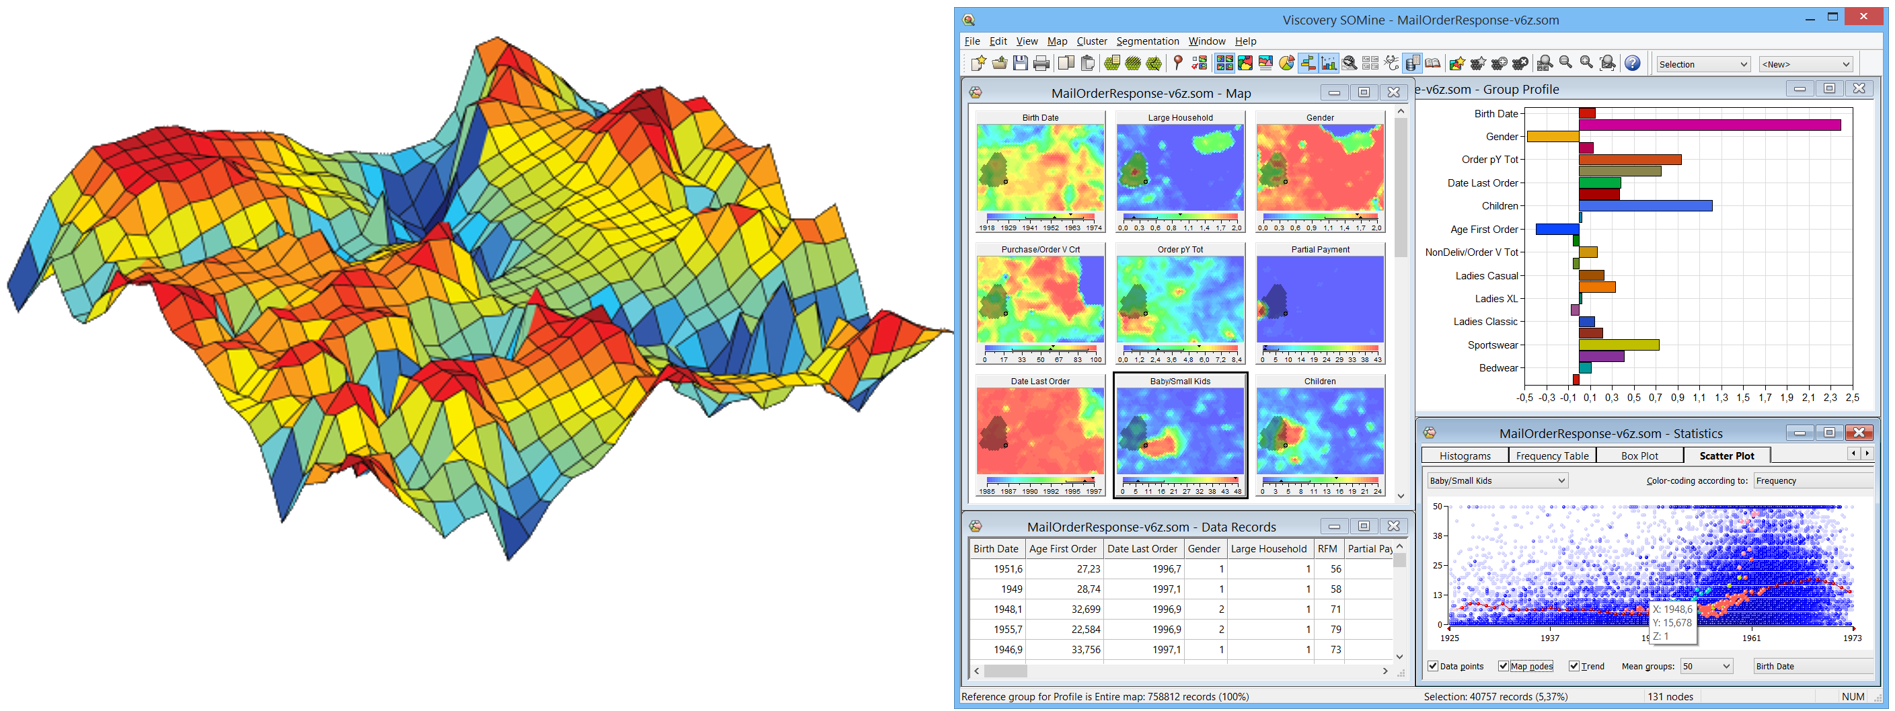
\includegraphics[width=\textwidth]{assets/nn/bb__som_ex2.png}
    \subcaption*{Natural grouping of instances in the two-dimensional grid (each cell colored using any of the features)}
  \end{subfigure}
  
  \caption{Unsupervised learning: SOMs}
  \label{fig:6_bb_som}
\end{figure}




